\chapter{Orbital Stability, Station-Keeping and Resonant Orbit Lifetime}
\label{app:station_keeping}

The 1-day and 7-day propagation results (Sections~\ref{sec:seed_1day_propagation} and~\ref{sec:seed_7day_propagation}) demonstrate that the RGTO seed orbit $\vec{\mathbf{A}}^{\,\mathrm{RGTO}^{\,2}}{}_{0,\,\mathrm{Coimbra}}$ maintains its repeating ground-track pattern over short time scales.  This appendix extends the propagation to 30~days and one~year to characterize the onset and evolution of resonance drift under atmospheric drag until the deorbiting of the satellite, introduces a simplified station-keeping algorithm implemented in NASA GMAT, and determines the uncontrolled orbital lifetime.

\section{Analysis Goals andSpacecraft and Propagation Configuration}\label{sec:sk_spacecraft_config}

The objective of this analysis is threefold: (i)~to determine how long the repeating ground-track condition is preserved---i.e.\ how many days the satellite continues to deliver the four-pass daily observation pattern over the core study domain $\mathcal{D}_{\mathrm{core}}$---, (ii)~to evaluate whether a simple altitude-maintenance algorithm can restore the resonance when drag causes the orbit to decay below the design altitude.  The propagation runs from the nominal seed altitude of $h_0 \approx 488$\,km until the orbit decays to approximately $h_{\mathrm{EOL}} \approx 385$\,km, below which the resonance condition can no longer be recovered and the satellite enters the end-of-life regime, and (iii)~to assess orbital lifetime of the satellite with vector $\vec{\mathbf{A}}^{\,\mathrm{RGTO}^{\,2}}{}_{0,\,\mathrm{Coimbra}}$ under the influence of atmospheric drag.

The satellite is modelled as a representative 12U CubeSat with the following physical parameters: dry mass $m = 18$\,kg, drag coefficient $C_D = 2.2$, coefficient of reflectivity $C_R = 1.3$, drag cross-sectional area $A_{\mathrm{drag}} = 0.1$\,m$^2$, and solar radiation pressure (SRP) area $A_{\mathrm{SRP}} = 0.5$\,m$^2$.  A spherical drag model is adopted.  The atmospheric density is computed using the Jacchia-Roberts model in its standard GMAT configuration, while the gravitational and non-gravitational force models are those described in the preceding analysis (Sec.~\ref{sec:perturbed_orbital_elements}).

\section{Uncontrolled Propagation: 30-Day and 1-Year Results}\label{sec:sk_uncontrolled}

\subsection{30-Day Propagation}

Figure~\ref{fig:RGTO_maps_Coimbra_Thirty_days} extends the ground-track and sky-plot analysis to 30~days without station-keeping.  The same observation-link metrics used for the 1-day and 7-day windows (Figs.~\ref{fig:RGTO_maps_Coimbra_One_day}--\ref{fig:RGTO_metrics_Coimbra_Seven_days}) are evaluated here.  The four-pass daily pattern persists during the first days, and the observation-link condition is still satisfied: the pass quality remains acceptable, with off-nadir angle minima close to $\sim\!10^{\circ}$ (indicating near-nadir overhead passes) and elevations above the $\varepsilon_{\min} = 15^{\circ}$ mask.  However, toward the end of the 30-day window the elevation peaks begin to decrease and some passes drift toward lower quality, suggesting the onset of resonance departure as the semi-major axis decays under drag.

\begin{figure}
    \centering
    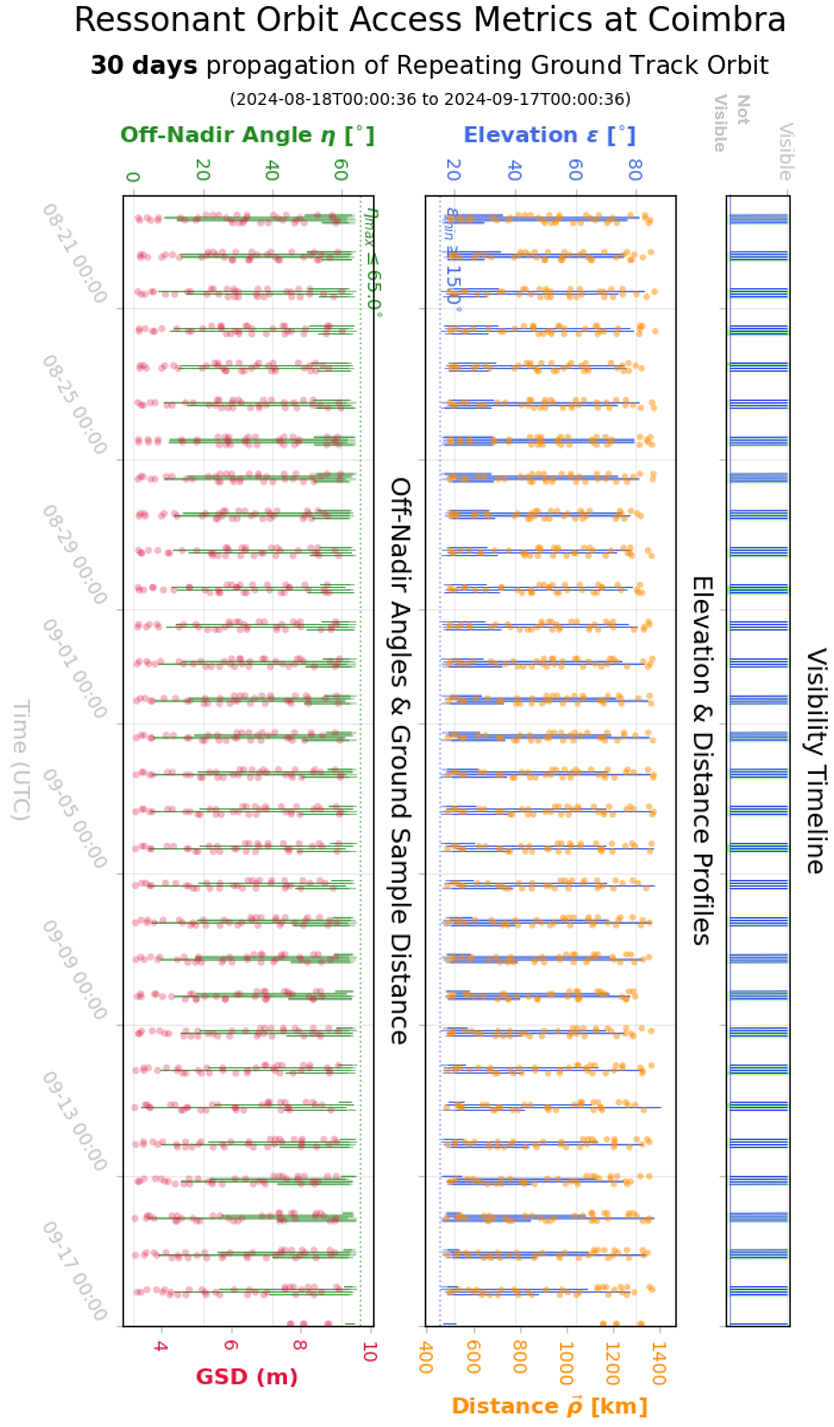
\includegraphics[width=0.8\linewidth]{images/RGTO_maps_Coimbra_Thirty_days.png}
    \caption{\footnotesize{Observation metrics of 30-day uncontrolled RGTO seed propagation over Coimbra ($\tau=15/1$, $h \approx 488$\,km). The four-pass daily pattern persists but elevation and off-nadir metrics begin to degrade toward day~30, indicating the onset of resonance drift.}}
    \label{fig:RGTO_maps_Coimbra_Thirty_days}
\end{figure}

\subsection{1-Year Uncontrolled Propagation}

To quantify the long-term resonance departure, the propagation is extended to one year without any orbit-maintenance manoeuvres.  Figure~\ref{fig:stationkeeping_Off} presents the orbital-element evolution over this period.  The semi-major axis decreases monotonically under atmospheric drag, and the repeating ground-track condition is progressively lost: the sub-satellite trace drifts across all longitudes, and the satellite ground track ceases to be confined to the Coimbra latitude band.  At the end of one year the orbit no longer bears any resemblance to the original resonance pattern. The satellite effectively covers the globe rather than revisiting the target domain.

This result confirms that uncontrolled drag is incompatible with sustained RGTO resonance and motivates the station-keeping strategy introduced in the next section.

\begin{figure}[H]
    \centering
    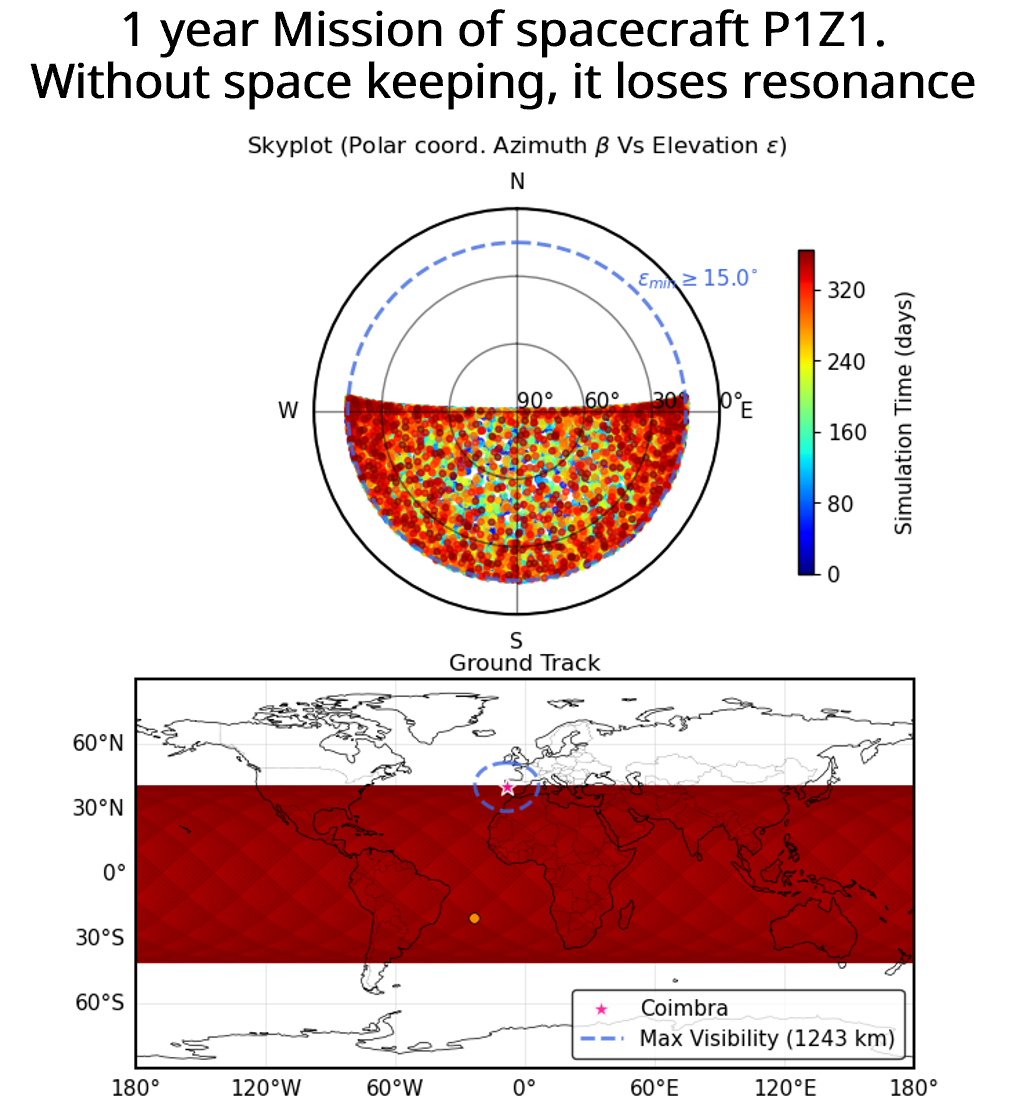
\includegraphics[width=0.8\linewidth]{images/stationkeeping_Off.png}
    \caption{\footnotesize{Orbital-element evolution over 1~year without station-keeping for the RGTO seed orbit.  Atmospheric drag causes a semi-major axis decay, leading to complete loss of the repeating ground-track resonance.}}
    \label{fig:stationkeeping_Off}
\end{figure}

\section{Station-Keeping Method and Results}\label{sec:sk_method}

A simplified altitude-maintenance algorithm is implemented in NASA GMAT to evaluate whether the RGTO resonance can be preserved over the mission lifetime.  The algorithm, illustrated in Fig.~\ref{fig:station_keeping_GMAT_algorithm}, operates as follows.  During the one-year propagation, the spacecraft altitude is continuously monitored.  When the altitude drops below the threshold $h_{\mathrm{thr}} = 480$\,km due to atmospheric drag, the algorithm is triggered:
\begin{enumerate}
    \item The satellite is propagated forward until it crosses the target latitude $\phi_{\mathrm{lat}} = 40.2^{\circ}$\,N (the Coimbra resonance latitude).
    \item At this position, an impulsive prograde burn ($\Delta V_1$) is applied to raise the orbit to approximately $h \approx 488$\,km.
    \item The orbital propagation continues until the subsequent apoapsis, where a second impulsive burn ($\Delta V_2$) circularises the orbit, restoring near-zero eccentricity.
\end{enumerate}
This two-burn sequence restores an orbit close to the original seed conditions.  The algorithm then resumes passive propagation until the next threshold crossing.  Note that an ideal impulsive-burn model is assumed: no propellant mass decrement is applied, and the spacecraft mass remains constant throughout.  A more detailed propulsion trade-off---including fuel budget, thruster sizing, and the impact of finite-burn duration---is deferred to future work.

\begin{figure}[H]
    \centering
    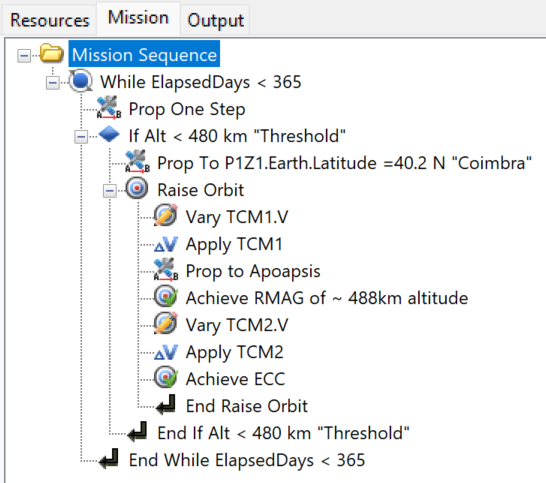
\includegraphics[width=0.4\linewidth]{images/station_keeping_GMAT_algorithm.png}
    \caption{\footnotesize{Simplified station-keeping algorithm implemented in GMAT.  When $h < 480$\,km, the spacecraft propagates to latitude $\phi = 40.2^{\circ}$, applies a prograde burn to raise the apoapsis to $\sim$488\,km, then circularises at apoapsis.}}
    \label{fig:station_keeping_GMAT_algorithm}
\end{figure}

Using this method, the same spacecraft and force-model configuration is propagated for one year under the same initial conditions as the uncontrolled case (Fig.~\ref{fig:stationkeeping_Off}).  The resulting orbital-element evolution is shown in Fig.~\ref{fig:stationkeeping_On}.  The resonance pattern is substantially better preserved compared with the uncontrolled case: the ground track remains concentrated around the Coimbra latitude band, and the four-pass daily observation sequence is largely maintained.  Residual drift is still visible, suggesting that the algorithm could be refined, but the result demonstrates that it is feasible to sustain the RGTO resonance with a simple low-thrust strategy.

\begin{figure}[H]
    \centering
    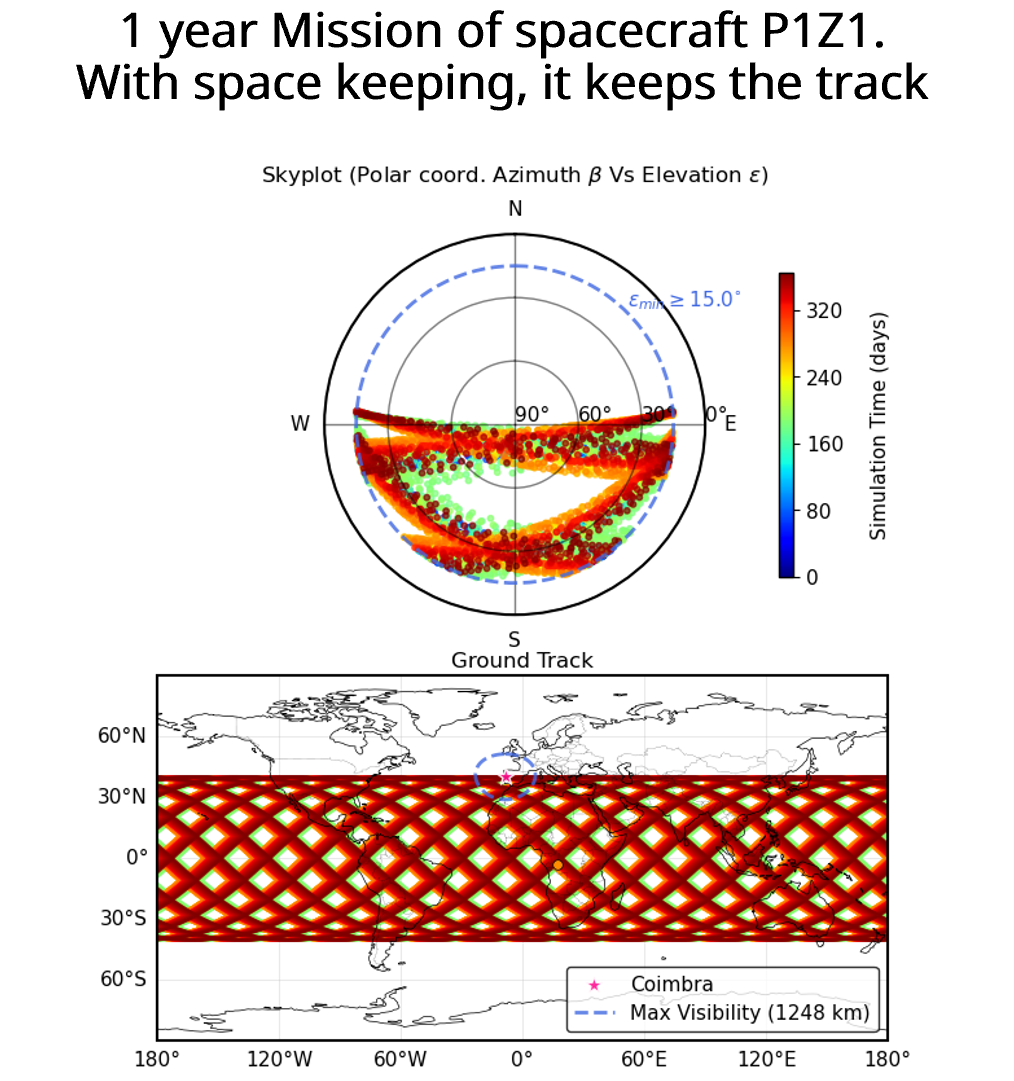
\includegraphics[width=0.8\linewidth]{images/stationkeeping_On.png}
    \caption{\footnotesize{Orbital-element evolution over 1~year with the station-keeping algorithm enabled.  The repeating ground-track resonance is substantially preserved; residual drift suggests the algorithm could be further refined.}}
    \label{fig:stationkeeping_On}
\end{figure}

\section{Altitude Evolution and End-of-Life Results}\label{sec:sk_altitude_eol}

Figure~\ref{fig:stationkeepingOn_hVSt} shows the altitude history for the one-year station-kept propagation.  Four burn events occur during the year, each triggered when $h$ drops below 480\,km.  After each two-burn correction the altitude is restored to $\sim$488\,km, and between burns the altitude remains above $\sim$482.5\,km.  This confirms that the simplified algorithm is sufficient to maintain the resonance altitude band over a one-year period with only four manoeuvre pairs per year.

\begin{figure}[H]
    \centering
    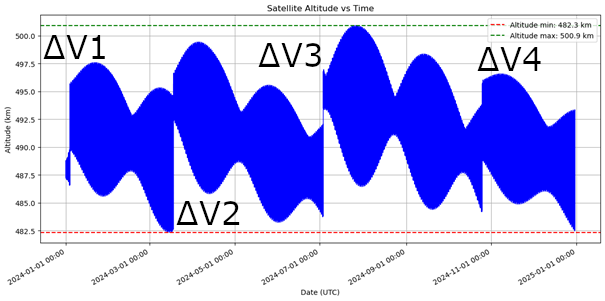
\includegraphics[width=0.75\linewidth]{images/stationkeepingOn_hVSt.png}
    \caption{\footnotesize{Altitude vs.\ time over 1~year with station-keeping.  Four burn events (triggered at $h < 480$\,km) restore the orbit to $\sim$488\,km; between burns the altitude remains above $\sim$482.5\,km.}}
    \label{fig:stationkeepingOn_hVSt}
\end{figure}

\subsubsection{Lifetime of Resonant Orbit}
Figure~\ref{fig:deorbiting_RGTO_Coimbra} presents the uncontrolled altitude decay from the initial $h_0 \approx 488$\,km.  Without station-keeping, the drag-induced descent accelerates as the spacecraft enters denser atmospheric layers, and the orbit reaches the end-of-life altitude ($h_{\mathrm{EOL}} \approx 285$\,km) after approximately 2.68~years.  This constitutes the natural orbital lifetime of the RGTO seed orbit for the assumed spacecraft parameters.


\begin{figure}[H]
    \centering
    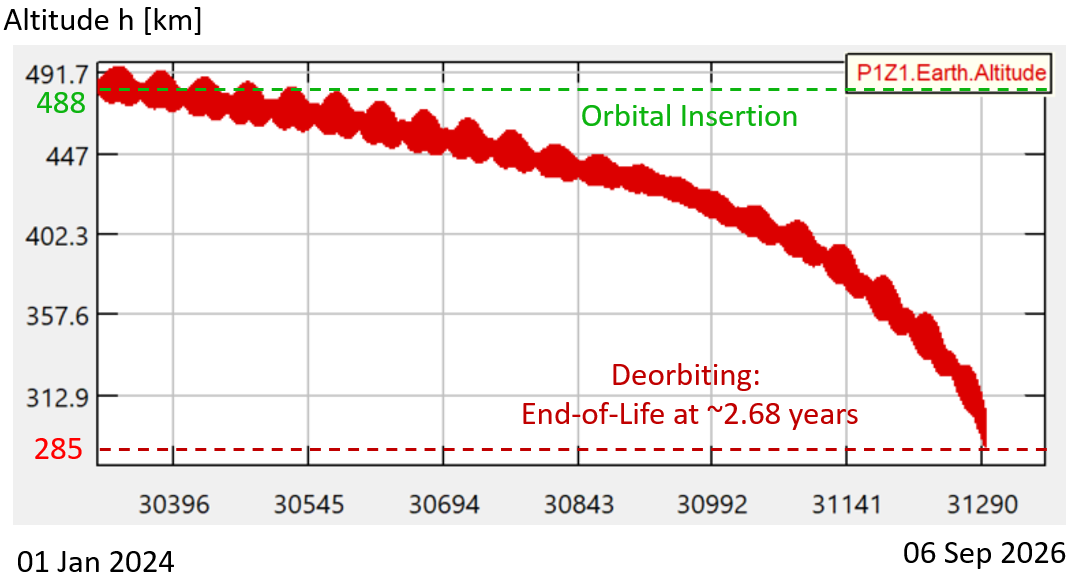
\includegraphics[width=0.6\linewidth]{images/deorbiting_RGTO_Coimbra.png}
    \caption{\footnotesize{Orbital altitude decay of object P1Z1 plotted against the UTC Modified Julian Date. The data illustrates the trajectory from an initial orbital insertion at $h = 488$ km on 01 Jan 202 (UTC) down to a final deorbiting altitude of 285 km on 06 Sep 2026 (UTC), spanning a total timeframe of 979.5 days (approximately 2.68 years).}}
    \label{fig:deorbiting_RGTO_Coimbra}
\end{figure}




\section{Summary}

The analysis demonstrates that the RGTO seed orbit $\vec{\mathbf{A}}^{\,\mathrm{RGTO}^{\,2}}{}_{0,\,\mathrm{Coimbra}}$ maintains the repeating ground-track resonance for approximately 7--30~days under uncontrolled propagation before drag-induced drift degrades the observation pattern.  A simplified two-burn station-keeping algorithm, triggered when the altitude drops below 480\,km, successfully restores the resonance with only four correction events per year.  Without station-keeping, the uncontrolled orbital lifetime is approximately 2.68~years.  These results confirm that the RGTO resonance is operationally sustainable with modest propulsive, but station keeping function is mandatory in a spacecraft system to provide a cost effective mission.  This analysis effort provide the lifetime warranty for the constellation design developed in the main text.
